%\documentclass[preprint]{aastex} 
\documentclass[iop,floatfix]{emulateapj} 

\usepackage[breaklinks,colorlinks,urlcolor=blue,citecolor=blue,linkcolor=blue]{hyperref}
\usepackage{graphicx}
%\usepackage{apjfonts}
\usepackage{enumerate}
\usepackage{amsmath,amssymb}
\usepackage{bm}
\usepackage{color}
\usepackage[utf8]{inputenc}

%version-control tagging based off of github.com/bd-j/speccal
%%% This file is generated by Makefile.
\newcommand{\githash}{b3f5d1c}\newcommand{\gitdate}{2014-08-19}\newcommand{\gitauthor}{Ian Czekala}

\newcommand{\prob}{{\rm prob}}
\newcommand{\qN}{\{q_i\}_{i=1}^N}
\newcommand{\qM}{\{q_{im}\}_{i=1,m=0}^{N,M}}
\newcommand{\yN}{\{y_i\}_{i=1}^N}

\newcommand{\kms}{ \textrm{km s}^{-1} }

\newcommand{\vM}{\mathsf{M}}
\newcommand{\vD}{\mathsf{D}}
\newcommand{\vR}{\mathsf{R}}
\newcommand{\vC}{\mathsf{C}}
\newcommand{\fM}{ \vec{{\bm M}}}
\newcommand{\fMi}{M_i}
\newcommand{\fD}{ \vec{{\bm D}}}
\newcommand{\fDi}{D_i}
\newcommand{\fR}{ {\bm R}}
\newcommand{\dd}{\,{\rm d}}
\newcommand{\trans}{\mathsf{T}}
\newcommand{\Z}{[{\rm Fe}/{\rm H}]}
\newcommand{\A}{[\alpha/{\rm Fe}]}
\newcommand{\matern}{Mat\'{e}rn}
\newcommand{\HK}{$\textrm{H}_2$O-K2}

%Chebyshev coefficients RULE!
\newcommand{\cc}[2]{c_{#2}^{(#1)}} %echelle order first, then degree coefficient

%flux
\newcommand{\flam}{f_\lambda}

%\vt stands for ``vector theta''
\newcommand{\vt}{ {\bm \theta}}
\newcommand{\vT}{ {\bm \Theta}}

%\vp stands for ``vector phi''
\newcommand{\vp}{ {\bm \phi}}
\newcommand{\vP}{ {\bm \Phi}}

%\phi and \Phi are used for nuisance parameters
\newcommand{\cheb}{ \vp_{\mathsf{P}}}
\newcommand{\chebi}[1]{ \vp_{\textrm{Cheb}_{#1}}} %for signifying a specific order
\newcommand{\Cheb}{ \vP_{\textrm{Cheb}}}
\newcommand{\Chebi}[1]{ \vP_{\textrm{Cheb}_{\ne #1}}} %for specifying everything but a specific order
\newcommand{\cov}{ \vp_{\mathsf{C}}}
\newcommand{\covi}[1]{ \vp_{\textrm{cov}_{#1}}} %for signifying a specific order
\newcommand{\Cov}{ \vP_{\textrm{cov}}}
\newcommand{\Covi}[1]{ \vP_{\textrm{cov}_{\ne #1}}} %for specifying everything but a specific order

\newcommand{\allParameters}{\vT} %all parameters
\newcommand{\nuisanceParameters}{\vP} %all nuisance parameters

%kernel notation
\newcommand{\KK}{\mathcal{K}}
\newcommand{\Kglobal}{\KK^{\textrm{g}}}
\newcommand{\Klocal}{\KK^l}


\newcommand{\todo}[1]{ \textcolor{blue}{\\TODO: #1}}
\newcommand{\comm}[1]{ \textcolor{red}{SA: #1}}
\newcommand{\hili}[1]{ \textcolor{green}{#1}}

\shorttitle{Spectroscopic inference}
\shortauthors{Czekala et al.}

\begin{document}

\graphicspath{{figs/}}

\slugcomment{draft: \today{}}


\title{A Method for the Spectroscopic Inference of Stellar Parameters}
\author{Ian Czekala, Sean M.~Andrews, et al.}
\affil{Harvard-Smithsonian Center for Astrophysics, 60 Garden Street, Cambridge, MA 02138}
\email{iczekala@cfa.harvard.edu}

\begin{abstract}
An abstract needs to go here. \\
tbd \\
tbd \\
tbd \\
tbd \\
tbd \\
tbd \\
tbd \\
tbd \\
tbd \\
tbd \\
tbd
\end{abstract}
\keywords{stars: fundamental parameters --- methods: data analysis --- methods: statistical}


\section{Introduction} \label{sec:intro}

All astronomers recognize that spectroscopy offers a wealth of information that can help
characterize the properties of the observing target.  In the context of stellar astrophysics, 
spectroscopy plays many fundamental roles.  The relative strengths and widths of stellar absorption 
lines provide access to key parameters like effective temperature ($T_{\rm eff}$) and surface 
gravity ($\log g$), enabling model comparisons in the Hertzsprung-Russell diagram to estimate the 
masses and ages so crucial to understanding stellar evolution, as well as individual elemental (and 
molecular) abundances or the collective ``metallicity" (typically parameterized as [Fe/H]), 
facilitating study of the chemical hallmarks of different stellar populations.  With sufficient 
spectral resolution, the velocity content of a spectrum can convey crucial information about 
stellar rotation ($v \sin i$) and kinematics (e.g., association with a cluster or companion through 
the radial velocity, $v_z$).  While many fields benefit from the spectroscopic measurements of 
these stellar properties, there is acute interest in the exoplanet community.  There, all estimates 
of the planet properties are made {\it relative} to the host properties (e.g., the planet-to-host 
mass or radius {\it ratio} is constrained with the radial velocity or transit techniques, 
respectively).  Moreover, essential clues to the planet formation process are encapsulated in the 
dependences of planet frequency on host mass \citep[e.g.,][]{johnson07,howard10} and metallicity 
\citep[e.g.,][]{fischer05,buchhave14}.   
% SA: we ought to check with exoplanet people on these references. Can do later...

That said, the robust and quantitative extraction of physical (or empirical) parameters from an 
observed spectrum can be an extraordinary challenge.  Stellar models are ultimately required as a 
comparative benchmark to associate observed spectral features with the parameters of interest.  
Generating a synthetic model spectrum requires a complex numerical treatment of the stellar 
structure and radiative transfer through the atmosphere \citep[e.g.,][]{kurucz93,castelli04,
hauschildt99,husser13,paxton11}.  Detailed models calibrated to individual stars are important, but 
rare (e.g., the Sun, Vega); as such, these stellar models are relatively untested in large swaths 
of parameter-space.  Moreover, they necessarily include simplifications to treat complicated 
physical processes (e.g., convection) or computational limitations (e.g., geometry, boundary 
conditions), and often must rely on incomplete or inaccurate atomic and molecular information 
(e.g., oscillator strengths, opacities).  In principle, the models could be further improved with 
appropriate reference to spectroscopic datasets.  Nevertheless, they achieve a remarkable level of 
success in reproducing many key diagnostic features in stellar spectra.  

There are various well-tested techniques being used to compare these models with observed spectra 
and thereby infer basic stellar parameters; here we highlight three examples to illustrate some key 
ideas.  First is a straightforward empirical approach that relies on distilling an information-rich 
subset of the data, usually in the form of spectral line equivalent widths and/or local continuum 
shapes.  A combined sequence of the ratios of these quantities are found to be especially sensitive 
to one key parameter in the models, and therefore can be used to quantify it 
\citep[e.g.,][]{gray94,reid95,rojas-ayala10,rojas-ayala12}.  This index comparison approach has 
the advantage of being trivially fast, but each index relationship is only informative over a 
limited region of parameter-space.  A second technique exploits the cross-correlation of an 
observed spectrum with a suite of model templates to identify an optimized set of parameters, 
usually with some weighting applied to specific spectral regions \citep[e.g., {\tt 
SPC};][]{buchhave12}.  In this case, the speed advantage is maintained and more data content is 
used (particularly in the spectral dimension), thereby achieving higher precision even for data 
with comparatively low sensitivity; the disadvantage is that the model quality and parameter 
inferences are assessed in an empirical, rather than probabilistic, framework.  A third approach 
employs a direct, pixel-by-pixel comparison between model and data, and is usually associated with 
a spectral synthesis back-end (e.g., {\tt MOOG}; \citealt{sneden73}; {\tt SME}; 
\citealt{valenti96}).  This technique has the benefits of parametric flexibility (e.g., one can fit 
for arbitrary abundances or structures) and a proper inference framework \citep[usually a 
least-squares approach, although increasingly in a Bayesian format;][]{shkedy07,schoenrich13}, but 
it is computationally expensive and can be biased by systematics \citep[e.g.,][]{mann13}; in 
practice, this often requires an effort focused on a pre-selected subsample of the data. 

In this article, we design a flexible forward-modeling approach to the general spectroscopic 
inference problem in a Bayesian framework, building on the best aspects of the latter two methods 
highlighted above.  Employing a non-trivial covariance matrix parameterized by both global 
(stationary) and local (non-stationary) Gaussian process kernels, we are able to account for 
residual pixel-to-pixel correlations that arise when comparing observed spectra to intrinsically 
imperfect models.  This approach minimizes the potential for bias, efficiently propagates 
systematic uncertainties into the parameter inferences, and ultimately can serve as tool for using
observations to guide substantially improvements in the models themselves.  An overview of the 
methodology of this approach is provided in Section \ref{sec:method}, including the covariance 
matrix formalism.  Some tests and example applications (for a high resolution optical spectrum of 
an F star, and a medium-resolution near-infrared spectrum of a mid-M star) of the method are 
described in Section \ref{sec:examples}.  Finally, a discussion of the potential utility of the 
technique, and the possibility of extending it to develop data-driven spectral models, is provided 
in Section \ref{sec:discussion}.  \\



\section{Methodology} \label{sec:method}

In this Section, we describe a generative Bayesian modeling framework that confronts some of the 
key obstacles in the spectroscopic inference problem.  The goal of this approach is to 
conservatively extract the maximal amount of information about a prescribed (and usually 
degenerate) parameter set by forward-modeling an observed spectrum, while also recognizing and 
explicitly accounting for the covariances and biases introduced by pathologically imperfect 
models.  The method is modular, and therefore can easily incorporate additional physical or 
nuisance parameters as desired without sacrificing an accurate reflection of the limitations in the 
data.  Moreover, with a well-crafted observational sample, this data-driven approach should 
ultimately enable us to systematically learn how synthetic spectral models can be improved.  The 
specific applications discussed here are related to the spectra of individual stars, but the 
methodology is generic (and could be used for the composite spectra of unresolved stellar clusters, 
galaxies, etc.).  

The remainder of this Section describes the mechanics of this modeling framework.  First, a model 
spectrum is generated for a given set of physical parameters (Section \ref{subsec:synthetic}), and 
then post-processed to mimic reality using a set of observational and practical nuisance parameters 
(Section \ref{subsec:postprocess}).  Next, a direct, pixel-by-pixel comparison between the data and 
model spectra is made with a prescribed likelihood function and a parametric treatment of the 
covariances between pixel residuals (Section \ref{subsec:likelihood}).  That process is iterated 
under the guise of hierarchical Markov Chain Monte Carlo (MCMC) simulations to numerically explore 
the posterior probability density of the model conditioned on the data, and thereby to determine 
constraints on the parameters of interest (Section \ref{subsec:MCMC}).  Along the way, these 
procedures are illustrated with real observations of the high resolution optical spectrum from a 
nearby F star.  That specific application, along with some alternative demonstrations of the 
method, are discussed in more detail in Section \ref{sec:examples}.


\subsection{Generating a Model Spectrum \label{subsec:synthetic}}

There are various approaches to synthesizing a spectrum, $f_{\lambda}$, for a specific set of model
parameters, $\vt_{\ast}$.  In an ideal case, a model stellar atmosphere is constructed and then 
subsequently processed through a radiative transfer code \citep[e.g.,][]{kurucz93,hauschildt99}.  
However, in general this approach is still computationally prohibitive for any iterative method of 
probabilistic inference.  One partial compromise is to interpolate over a library of atmosphere 
structures that were pre-computed for a discrete grid of parameter values, $\{\vt_{\ast}\}^{\rm 
grid}$, for some arbitrary $\vt_{\ast}$, and then perform a radiative transfer calculation with 
that interpolated atmosphere to synthesize $\flam$ \citep[e.g., as for {\tt SME};][]{valenti96}.  A 
more common variant is to instead rely on interpolation over a library of pre-synthesized model 
spectra, $\flam(\vt_{\ast})$ \citep[e.g.,][]{castelli04,allard12,husser13}.  While technically the 
former approach is most similar to the ideal case, the computational cost of repeated spectral 
synthesis is sufficiently high to make a detailed exploration of parameter space (particularly for 
data with a large spectral range) considerably less appealing.  An alternative approach eschews 
forward modeling entirely (and therefore repeated spectral syntheses and/or library 
interpolations), and instead evaluates the models only at the discrete grid points of the library.  
Then, these discretized samples of the posterior probability density can be interpolated to an 
arbitrary $\vt_{\ast}$ to construct appropriate confidence intervals \citep[similar to the method 
of {\tt SPC};][]{buchhave12}.  The difficulty with this latter approach is that the parameter 
uncertainties can be smaller than the grid spacing; in that case, there is valid concern that this 
interpolation might not accurately recover intrinsic parameter degeneracies.

We opt for the computationally expedient approach that employs a library of model spectra, 
$\flam(\{\vt_{\ast}\}^{\rm grid})$, where $\vt_{\ast} = [T_{\rm eff}, \,\, \log{g}, \,\, 
[{\rm Fe/H}]]$.  However, it is worth noting that the techniques developed here are applicable to 
{\it any} ``back-end" that generates a model spectrum.  In our adopted approach, the model 
spectrum for an arbitrary $\vt_{\ast}$ is interpolated from a spectral library, 
\begin{equation} \label{eqn:interp}
\flam(\{\vt_{\ast}\}^{\rm grid}) \leadsto \flam(\vt_{\ast}),
\end{equation}
where we assign the symbol $\leadsto$ as an interpolation operator.  The multi-dimensional 
interpolation in Eq.~\ref{eqn:interp} needs to be performed many times, so computational efficiency 
is critical.  In practice, a simple tri-linear interpolation is suitably fast, but introduces an 
undesirable level of inaccuracy (particularly in the [Fe/H] dimension).  The interpolation quality 
can be empirically estimated by performing the operation in Eq.~\ref{eqn:interp} across a 
$\{\vt_{\ast}\}^{\rm grid}$ grid point, and then comparing the interpolated spectrum with the 
corresponding library spectrum.  After an extensive exploration of such calculations 
\citep[see also][]{husser12}, we concluded that this interpolation
technique is found to be accurate within a few percent per full-resolution
model pixel and $\lesssim 1$\% once the spectrum is downsampled to the pixels of the detector. Ideally,
this pre-interpolation could be avoided if the spectral library was computed
over a refined grid (with a substantial up-front computational investment); but
for the time being, we can empirically propagate these interpolation
uncertainties into the likelihood calculations (as will be described in 
Section~\ref{subsec:likelihood}).  

\subsection{Post-Processing} \label{subsec:postprocess}

Generally, the ``raw" model spectrum $\flam(\vt_{\ast})$ is highly over-sampled compared to the 
observed spectrum, and does not account for several additional observational and 
instrumental effects that become important in comparisons with real data.  Therefore, a certain 
amount of post-processing is required before assessing the model quality.  We treat that 
post-processing in two stages: the first deals with an additional set of ``observational" 
parameters, $\vt_{\rm obs}$, that incorporate dynamical effects, geometry, and the relative 
location of the target, while the second employs a suite of nuisance (hyper-)parameters ($\vp$) 
designed to mitigate an imperfect data calibration.

We can further divide $\vt_{\rm obs}$ into those parameters that impact the model primarily in the 
spectral or flux dimensions.  For the former, we consider three kernels that contribute to the 
line-of-sight velocity distribution function, $\varphi_v$.  The first, $\mathcal{F}_v^{\rm inst}$, 
treats the instrumental spectral broadening.\footnote{For computational efficiency, we first 
pre-convolve the entire raw spectral library with a slight under-prediction of $\mathcal{F}_v^{\rm 
inst}$ and resample the spectra to a lower resolution.  Because the instrumental point spread 
function acts as a low-pass filter, this procedure reduces the size of the library by a factor of 
10 or more while still preserving the final Fourier content of the spectra.  Then, when any given 
spectrum is post-processed, the actual $\mathcal{F}_v^{\rm inst}$ used is treated as a smaller 
``correction" to this pre-processing kernel.}  For illustrative purposes, we assume 
$\mathcal{F}_v^{\rm inst}$ is a Gaussian with mean $v = 0$ and constant width $\sigma_v$ at all 
$\lambda$, although more sophisticated forms could be adopted.  The second, $\mathcal{F}_v^{\rm 
rot}$, characterizes the broadening induced by (projected) stellar rotation, parameterized by 
$v\sin{i}$ as described by \citet[][his Eq.~18.14]{gray08}.  And the third, $\mathcal{F}_v^{\rm 
dop} = \delta(v-v_z)$, incorporates the radial velocity through a Doppler shift.  The model 
spectrum is modified by the parameters $[\sigma_v, \,\, v\sin{i}, \,\, v_z]$ through these kernels, 
using a convolution in velocity-space,\footnote{In practice, these convolutions are performed as 
multiplications in Fourier-space to better preserve spectral information \citep[cf.,][]{tonry79}; 
the mathematical formalism is presented for clarity.}
\begin{eqnarray} \label{eqn:broadening}
\flam(\vt_{\ast}, \sigma_v, v\sin{i}, v_z) &=& \flam(\vt_{\ast}) \otimes \varphi_v \\
                                           &=& \flam(\vt_{\ast}) \otimes \mathcal{F}_v^{\rm inst} \otimes \mathcal{F}_v^{\rm rot} \otimes \mathcal{F}_v^{\rm dop}, \nonumber
\end{eqnarray} 
and then re-sampled onto the discrete wavelengths corresponding to each data pixel, 
\begin{equation} \label{eqn:resampling}
\flam(\vt_{\ast},  \sigma_v, v\sin{i}, v_z) \mapsto \vM(\vt_{\ast},  \sigma_v, v\sin{i}, v_z),
\end{equation}
where the $\mapsto$ symbol denotes a re-sampling operator that maps the model spectrum onto the 
$N_{\rm pix}$-element model vector $\vM$ (and $N_{\rm pix}$ is the number of pixels in the 
spectrum).  Figure \ref{fig:broadening} shows a (condensed) graphical representation 
of these post-processing steps.

\begin{figure}[!t]
\begin{center}
  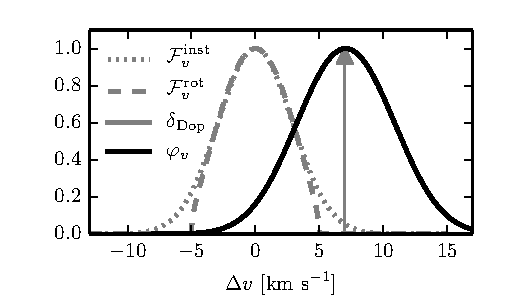
\includegraphics{figs/kernels.pdf}
  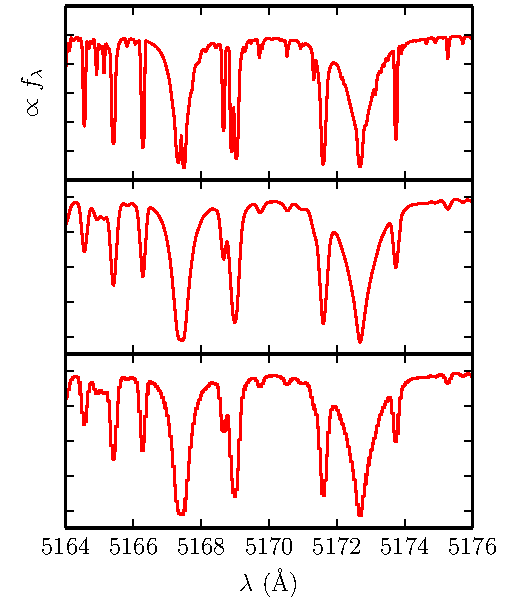
\includegraphics{figs/high2low.pdf}
  \figcaption{({\it top}) The line-of-sight velocity distribution function, $\varphi_v$, and its 
decomposition into broadening kernels.  The instrumental kernel ({\it dotted}) is treated as 
a Gaussian, the rotation kernel ({\it dashed}) is a Gaussian-like function of the projected 
rotational velocity, and the Doppler kernel ({\it solid}) is a $\delta$-function that introduces 
the radial velocity.  In this specific case, $\sigma_v = 2.9$\,km s$^{-1}$, $v\sin{i} = 5$\,km 
s$^{-1}$, and $v_z = 7$\,km s$^{-1}$, appropriate for the example in Section \ref{sec:examples}.x.
({\it bottom}) A segment of a raw, full-resolution model spectrum and its post-processed equivalent 
after convolution by $\varphi_v$ and re-sampling at the coarser resolution of the detector pixels. 
\label{fig:broadening}}
\end{center}
\end{figure}

At this stage, the model is further modified in the flux dimension.  A typical synthetic spectrum 
is computed as the flux that would be measured {\it at the stellar surface}, and so needs to be 
diluted by the subtended solid angle, $\Omega = (R_{\ast}/d)^2$, where $R_{\ast}$ is the stellar 
radius and $d$ is the distance.  An additional wavelength-dependent scaling factor is applied to 
account for interstellar extinction, assuming some previously-derived extinction law $A_{\lambda}$ 
\citep[e.g.,][]{cardelli89} that is parameterized by $A_V$.  The parameters $[\Omega, \,\, A_V]$ 
are then applied as
\begin{eqnarray} \label{eqn:scaling}
\vM(\vT) &=& \vM(\vt_{\ast}, \vt_{\rm obs}) \\
         &=& \vM(\vt_{\ast}, \sigma_v, v\sin{i}, v_z) \times \Omega \times 10^{-0.4\,A_{\lambda}}, \nonumber
\end{eqnarray}
with simplified notation such that $\vT \equiv [\vt_{\ast}, \,\, \vt_{\rm obs}]$, 
where $\vt_{\rm obs} = [\sigma_v, v\sin{i}, v_z, \Omega, A_V]$.

The procedure so far, summarized in Eq.~\ref{eqn:interp}--\ref{eqn:scaling}, is composed of 
straightforward operations demanded by practical astronomical and computing issues.  If the data 
were {\it perfectly} calibrated, we could proceed to a likelihood calculation that makes a direct 
comparison with $\vM(\vT)$.  However, that is unlikely to be the case.  The key concern is that an 
imperfect calibration might produce mismatches in the underlying shapes of the data and model.  
Although such mismatches presumably occur at a low-level over relatively broad wavelength scales, 
they still might represent a non-trivial likelihood contribution, and thereby bias our estimates of 
the physical parameters.  This concern is usually treated externally to any modeling procedure, most often 
by dividing the observed spectrum (and model spectrum) by a polynomial in $\lambda$.  But that 
``normalization" implicitly assumes that there is no relevant information content in the spectral 
shape; if $\vT$ also contributes on the mismatched scales, then adopting this approach will corrupt 
the inferences of these parameters.  Moreover, in practice this approach is limited, since defining 
an appropriate polynomial becomes difficult in cases where the spectral line density is high (e.g., 
molecular bands for cool stars).  

We employ an analogous, but more rigorous, approach to deal with this issue, cast {\it internal} to 
the modeling framework to propagate the uncertainties introduced by additional degrees of freedom 
in the model.  Deviations in the spectral shape introduced by calibration residuals are treated as 
explicit contributions to the model spectrum, enabling an exploration of the distribution of 
possible ``tweaks" to the calibration that can be compartmentalized into a set of nuisance 
parameters and then marginalized.  This way, the inferences for the stellar parameters will 
properly account for the underlying uncertainty in the calibration of the spectral shape.  In 
practice, this is achieved by distorting segments of the model spectrum with polynomials, 
$\mathsf{P}$ \citep[e.g.,][]{eisenstein06,koleva09}.  For data that has $N_{\rm ord}$ spectral 
orders, each denoted with index $o$, the model spectrum can be decomposed into the set of orders
\begin{eqnarray} \label{eqn:chebyshev}
\vM(\vT, \cheb) &=& \{ \vM_o(\vT) \times \mathsf{P}_o \} \\
                &=& \{ \vM_o(\vT) \times \sum_n c_o^{(n)} \, T_o^{(n)} \}, \nonumber
\end{eqnarray}
and $T^{(n)}$ is the $n^{\rm th}$ degree Chebyshev function.  The $n \times N_{\rm ord}$ 
coefficients are considered a set of nuisance (hyper-)parameters, $\cheb = [\{c_o^{(0)}, c_o^{(1)}, 
\ldots, c_o^{(n-1)} \}]$.  With judicious priors, we can ensure that the unintended treatment of 
real spectral features (e.g., molecular bands) as residual calibration artifacts is negligible.  
The lowest-degree (scaling) coefficient, $c^{(0)}$, is naturally degenerate with the solid angle, 
$\Omega$.  Therefore, we enforce an additional constraint that the mean of the polynomial is 
unity.  For data with a single spectral order, this means simply setting $c^{(0)} = 1$.  In the 
multiple order case, we assign $c^{(0)} = 1$ in an arbitrary order as an anchor, but permit the 
$c^{(0)}$ in other orders to be different.  It is worth noting that this formalism can, in 
principle, be extended to develop models for completely uncalibrated spectra, rather than the 
residual calibration mismatches described here (with a suitable relaxation of the priors on 
$\cheb$).  Figure \ref{fig:chebyshev} offers a practical demonstration of how these nuisance 
parameters are applied. 

\begin{figure}[!b]
\begin{center}
  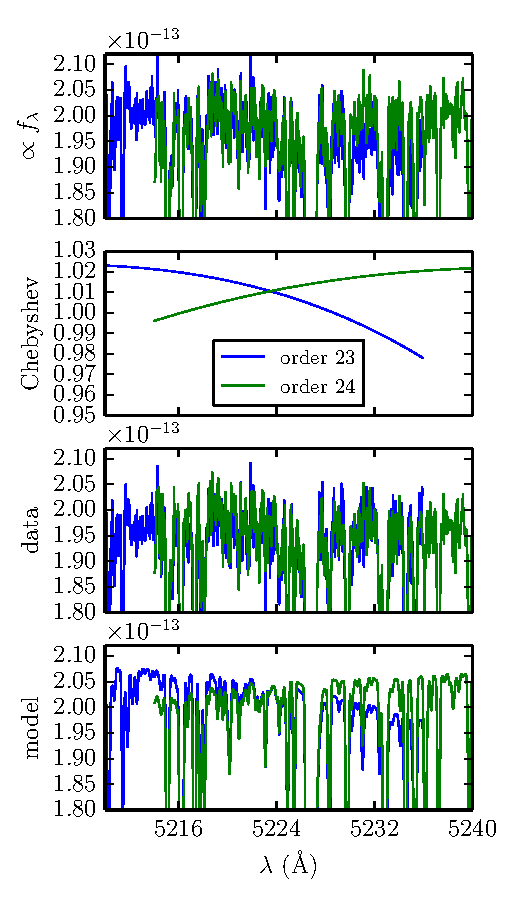
\includegraphics{figs/chebyshev.pdf}
  \figcaption{
The spectrum at the overlap of two echelle orders (23 \& 24). \textbf{Panel 1}: The flux-calibrated dataset shows a slight discrepancy of $\lesssim 3$\% between orders. \textbf{Panel 2}: To account for this residual error in the flux calibration, we multiply the model spectrum by a Chebyshev polynomial, whose coefficients are parameters that are part of the model. \textbf{Panels 3 \& 4}: In principle, we could divide the data by these polynomials to recover what the true flux-calibrated data should be (panel 3), but instead we multiply the model by the polynomials to recover the original discrepancy between orders (panel 4). This has the advantage of preserving the original dataset as a fixed quantity and makes the model (Equation~\ref{eqn:chebyshev}) linear in the Chebyshev polynomial coefficients.
\label{fig:chebyshev}}
\end{center}
\end{figure}


\subsection{Model Evaluation} \label{subsec:likelihood}

The quality of the model spectrum is assessed by comparing to the data with a pixel-by-pixel 
likelihood calculation.  If we denote the data spectrum as $\vD$, then a corresponding residual 
spectrum (an $N_{\rm pix}$-element vector) can be defined for any input parameter set,
\begin{equation}
\vR \equiv \vR(\vT, \cheb) \equiv \vD-\vM(\vT, \cheb).
\end{equation}
To quantify the probability of the data conditioned on the model, we adopt a standard 
multi-dimensional Gaussian likelihood function
\begin{equation}
p(\vD|\vM) =  \frac{1}{[(2 \pi)^{N_{\rm pix}} \det(\vC)]^{1/2}} \exp\left ( -\frac{1}{2} \,
   \vR^\trans \vC^{-1} \vR \right )
   \label{eqn:likelihood}
\end{equation}
that penalizes models which yield larger residuals and explicitly allows for covariances in the 
residual spectrum through the $N_{\rm pix} \times N_{\rm pix}$ matrix $\vC$.  For practical 
reasons, the log-likelihood is used as the quality metric, where
\begin{equation}
  \ln{p(\vD | \vM)} = -\frac{1}{2} \left( \vR^\trans \vC^{-1} \vR + \ln{\det{\vC}} + N_{\rm pix} \ln{2\pi} \right).
  \label{eqn:lnlikelihood}
\end{equation}

The covariance matrix $\vC$ characterizes both the measurement uncertainty ($\sigma$; ``noise") in 
each pixel and the intrinsic covariance between pixels.  The special case where each pixel 
represents an independent measurement results in a diagonal covariance matrix, $\vC_{ij} = 
\delta_{ij} \,\, \sigma_i$ where $\sigma_i$ is the uncertainty in pixel $i$ and $\delta_{ij}$ is 
the Kronecker delta function, and Eq.~\ref{eqn:lnlikelihood} reduces to the familiar
\begin{equation}
\ln{p(\vD | \vM)} = -\frac{1}{2} \sum_i^{N_{\rm pix}} \frac{\vR_i^2}{\sigma_i^2} \equiv -\frac{\chi^2}{2},
\label{eqn:chisq}
\end{equation}
the sum of the square of the residuals weighted by their inverse variances.  However, the problem 
being addressed here necessitates the use of a more complex covariance matrix; additional 
off-diagonal terms that can explicitly characterize (1) pixel-to-pixel covariances imposed by the 
discrete over-sampling of the line-spread function, and (2) highly correlated residuals as 
manifestations of the still-imperfect model library are required to avoid biasing our inferences of 
the physically interesting parameters ($\vT$).  The following subsections describe how these issues 
are addressed in the practical implementation of $\vC$.  


\subsubsection{Global Covariance Structure} \label{subsec:global_covariance}

Astronomical spectrographs are designed such that the detector over-samples the instrumental 
line-spread function with at least a few pixels.  Therefore, adjacent pixels never record 
completely independent samples of the true spectrum.  In that case, a difference between an 
observed and modeled spectral feature will create a correlated residual that spans multiple 
pixels.  This can be demonstrated practically through the autocorrelation of $\vR$: a slight model 
mismatch will produce correlated residuals over a characteristic scale similar to the instrumental
broadening kernel width ($\sigma_v$).  Figure \ref{fig:class0} highlights a specific example of 
these correlated residuals in real data; a significant autocorrelation signal is found on a $\sim$5 
pixel scale, corresponding to the 6.8\,km s$^{-1}$ FWHM of $\mathcal{F}_v^{\rm inst}$.  

\begin{figure}[!htb]
\begin{center}
  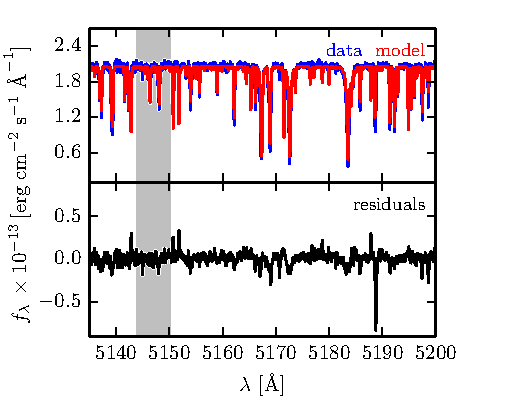
\includegraphics{residuals_23.pdf}
  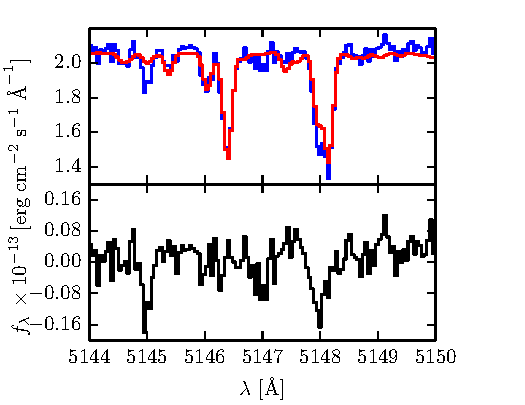
\includegraphics{class0_residuals.pdf}
  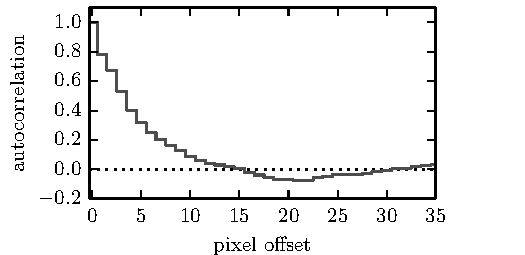
\includegraphics{class0_autocorrelation.pdf}
  \caption{\textbf{Top}: A typical model fit to a data spectrum, with
  parameters drawn from the posterior distribution, and the residuals that
  result. \textbf{Left} The low-amplitude, mildly covariant residuals enlarged
  to show the mildly covariant structure produced by slight mismatch between
  the data and model spectra.   \textbf{Right} The autocorrelation of the
residual sequence shown at left. Notice that there is significant correlation
for offsets of $\lesssim 5$ pixels.}
\label{fig:class0}
\end{center}
\end{figure}

It seems important to distinguish here between ``noise" and the fit residuals.  Noise introduced to 
the spectrograph by astrophysical or instrumental effects is generally uncorrelated with 
wavelength.  The arrival and propagation of each photon through the instrument and into the 
detector can be considered an independent event.  In essence, the noise itself is not correlated, 
but the fit residuals likely are.  However, from a mathematical perspective the correlated 
residuals can be treated in the same way as correlated noise, by constructing a non-trivial 
covariance matrix with off-diagonal terms.  In practice, this is achieved by parameterizing $\vC$ 
with a kernel that describes the covariance between any pair of pixels, indexed $ij$, representing 
wavelengths $\lambda_i$ and $\lambda_j$.

For a well-designed spectrograph and sufficiently accurate model, this {\it global} (i.e., present 
throughout the spectrum) covariant structure should have a relatively low amplitude and small 
correlation length.  To describe that structure, we use a stationary covariance kernel (or radial 
basis function) with an amplitude that depends only on the velocity distance between two pixels, 
\begin{equation}
  r_{ij} = r(\lambda_i, \lambda_j) = \Delta v = \frac{c}{2} \left | \frac{\lambda_i 
   - \lambda_j}{ \lambda_i + \lambda_j} \right |,
\end{equation}
where $c$ is the speed of light.  This parametric kernel describes the covariance between pixel 
residuals, 
\begin{equation}
  \Kglobal_{ij} =  \langle \vR_i \; \vR_j \rangle.
  \label{eqn:expectation}
\end{equation}
A variety of kernels have been used in the field of Gaussian processes to parameterize such a 
covariant structure \citep[e.g.,][]{rasmussen05}.  Here, we adopt the commonly-employed \matern\ 
kernel with $\nu = 3/2$,
\begin{equation}
  \Kglobal_{ij}(\vp_{{\mathsf C}, g}) = a_{\rm g} \left(1 + \frac{\sqrt{3}\, r_{ij}}{\ell} \right ) \exp 
   \left (- \frac{\sqrt{3}\, r_{ij}}{\ell} \right ),
   \label{eqn:global}
\end{equation}
where the (hyper-)parameters $\vp_{{\mathsf C}, g} = [a_g, \ell]$ include an amplitude ($a_g$) and 
scale ($\ell$).  To ensure that $\vC$ remains a relatively sparse matrix that 
enables computational expendiency, we employ a Hann window function
\begin{equation}
  w_{ij}^{\rm g} \,(r_0) = \left \{ 
    \begin{array}{cc}
    \frac{1}{2} + \frac{1}{2} \cos \left(\frac{\pi r_{ij}}{r_0} \right) & r_{ij} \le r_0 \\
    0 & r_{ij} > r_0 \\
  \end{array}
  \right .
  \label{eqn:Hann}
\end{equation}
to taper the kernel.  The truncation distance $r_0$ can be fixed to a reasonable multiple of the 
scale (we set $r_0 = 4\ell$).  Figure \ref{fig:matrix} demonstrates that random draws from such a 
kernel readily produce correlated structure similar to those seen in a typical residual spectrum.

\begin{figure*}[!htb]
\begin{center}
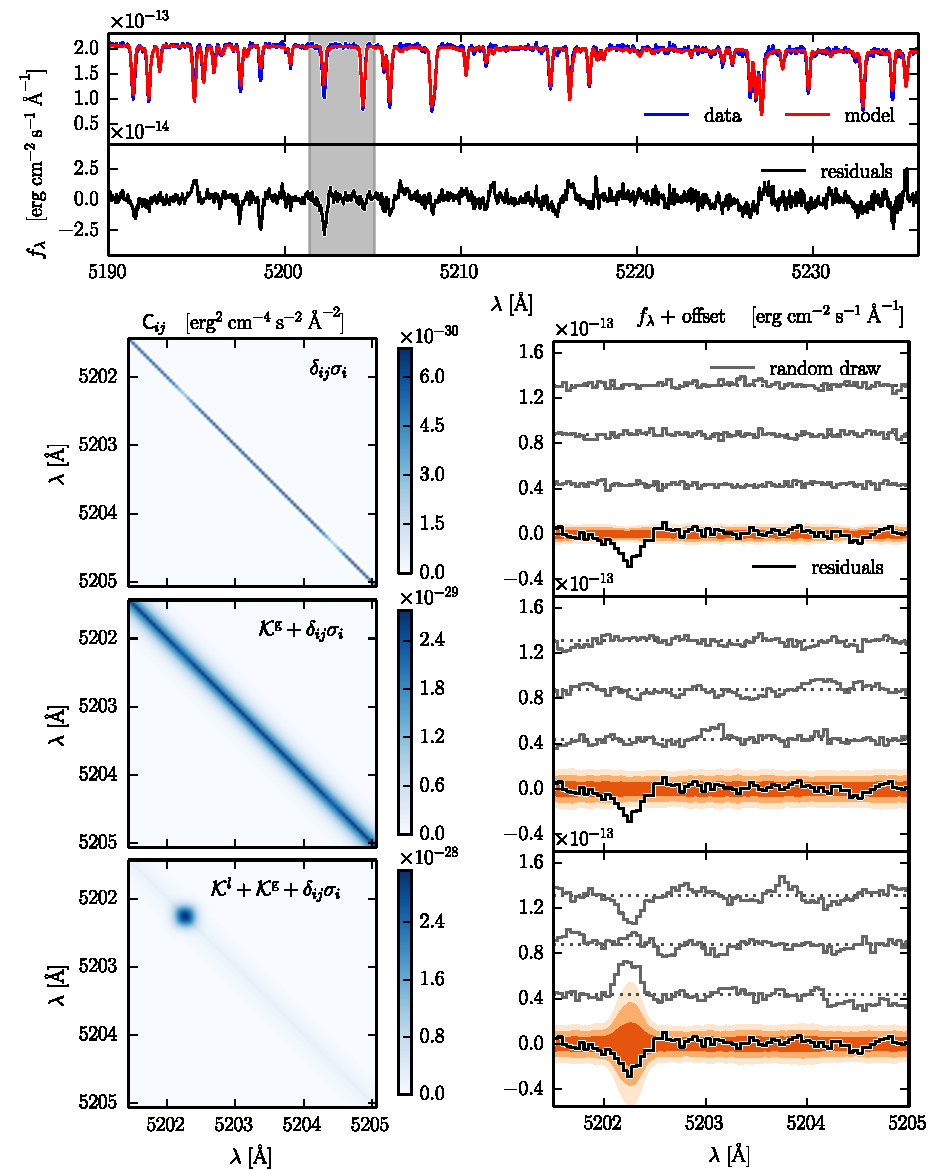
\includegraphics{figs/matrix_compilation.pdf}
\caption{\textbf{Top}: A typical model fit and residual spectrum with a demonstrative region shaded in grey, showing the scale and structure of the residuals. \textbf{Left column}: A small inset of the covariance matrix corresponding to the gray region. Note that the colorbar scale changes with each inset in order to best illustrate the structure of the matrix. \textbf{Right column}: Each panel shows three random draws (gray) from a multivariate normal distribution using the covariance matrix in the left column. At the bottom of each panel are the one, two, and three sigma contours (orange) of 200 random draws overlaid with the actual residuals from the gray region. \textbf{First row}: White, Poisson-only noise ($\delta_{ij}\sigma_i$) does a poor job of reproducing both the scale and structure of a typical residual spectrum. \textbf{Second row}: The addition of a global kernel ($\mathcal{K}^{\rm g}$) yields random draws that closely approximate the structure and amplitude of the residuals, but miss the strong outlier line at 5202.2 \AA. \textbf{Third row}: Finally, adding in a local kernel ($\mathcal{K}^l$) at the location of the outlier produces random draws that completely match the structure of the residuals. Interestingly, note that the covariance matrix can produce random draws that have negative, positive, and even flat residual lines. The point is that with a non-trivial covariance matrix, the likelihood function can now accommodate the residuals generated from a typical spectroscopic fit. Stated differently, random draws from the likelihood function can now produce behavior that looks like the residuals, whereas before with only white noise it could not. All parameters of the covariance kernels are determined self-consistently along with the stellar parameters. }
\label{fig:matrix}
\end{center}
\end{figure*}

\subsubsection{Local Covariance Structure} \label{subsec:local_covariance}

Aside from the global covariance structure, there can also be local regions of strong (highly 
correlated) residuals that need to be treated in the modeling framework.  These patches of large 
$\vR$ are usually produced by imperfect spectral lines in the models (missing opacity sources, 
uncertain oscillator strengths, etc.); some representative examples are highlighted in Figure 
\ref{fig:badlines}.  To parameterize such regions in $\vC$, we introduce a sequence of 
non-stationary kernels that explicitly depend on the actual wavelength values of a pair of pixels 
(on $\lambda_i$ and $\lambda_j$), and not simply the distance between them ($r_{ij}$).  

Assuming that these local residuals are produced primarily by pathological differences in the 
spectral line strength (rather than shape or center), a simple Gaussian is a reasonable residual 
model.  In that case, the $k^{\rm th}$ such local residual could be described as
\begin{equation}
\vR = a_k \exp \left[ - \frac{r^2(\lambda,\mu_k)}{2\sigma_k^2} \right],
\end{equation}
with peak amplitude $a_k$, mean wavelength $\mu_k$, and width $\sigma_k$.  Following 
Eq.~\ref{eqn:expectation}, the covariance of any two pixels related to the $k^{\rm th}$ local 
residual regions can be written
\begin{equation} \label{eqn:kregion}
  \mathcal{K}^{l,k}_{ij} = a_k^2 \exp \left [ - \, \frac{r^2(\lambda_i, \mu_k) + r^2(\lambda_j, \mu_k)}{2 \sigma_k^2}\right ],
\end{equation}
such that the full local covariance kernel composed of a sequence of residual regions is the linear 
combination,
\begin{equation} \label{eqn:klocal}
\Klocal_{ij}(\vp_{{\mathsf C},l}) = \sum_k w^k_{ij} \, \mathcal{K}^{l,k}_{ij},
\end{equation}
with a set of (hyper-)parameters $\vp_{{\mathsf C},l} = [\{a_k, \mu_k, \sigma_k\}]$.  Note that we 
again taper the kernels with Hann windows (Eq.~\ref{eqn:Hann}) to ensure a sparse covariance 
matrix; in this case, the truncation distance $r_0$ can be set to some multiple of the Gaussian 
width (we use $r_0 = 4\sigma_k$).  Figure \ref{fig:matrix} shows how this non-stationary Gaussian 
kernel generates a localized region of enhanced variance that successfully mimics the kind of 
residuals produced by an inaccurate spectral line model.  In effect, these kernels down-weight the 
influence of such strong residuals in the likelihood calculation, mitigating any potential bias 
they might induce on inferences of the interesting parameters ($\vT$).  This acts like a robust, 
flexible, and unbiased method for (correlated) outlier rejection that preserves the integrity of 
the probabilistic framework (as opposed to manual or threshold-based clipping or masking).  

These local kernels can be further modified to account for more complex residual structures.  For 
example, late-type stars with imperfectly modeled molecular bandheads may produce a complicated 
pattern of positive and negative residuals or a pronounced mismatch over a relatively large 
spectral scale.  This phenomenologically different local covariance behavior can still be treated 
in this framework if we design an appropriate kernel. 


\subsubsection{Composite Covariance Matrix}

We can now compute the covariance matrix employed in the likelihood calculation 
(Eq.~\ref{eqn:lnlikelihood}) as the linear combination of the trivial pixel-by-pixel noise matrix 
and these global and local kernels, 
\begin{equation}
\vC_{ij}(\cov)  = b \, \delta_{ij} \, \sigma_i + w_{ij} \,\, \Kglobal_{ij}(\vp_{{\mathsf C}, g}) + 
                  \Klocal_{ij}(\vp_{{\mathsf C}, l}), 
\end{equation}
with (hyper-)parameters $\cov = [\vp_{{\mathsf C}, g}, \vp_{{\mathsf C}, l}]$.  The factor $b$ is 
a (constant) parameter that scales up the pixel noise values to account for additional detector or 
data reduction uncertainties (e.g., read noise, uncertainties in the spectral extraction procedure, 
and interpolation errors); reasonable values are $b \approx 1.02$--1.10 for well-calibrated optical 
spectra (see Section \ref{sec:examples} for examples).  If there are $N_{\rm loc}$ local covariance 
patches (see Section \ref{subsec:MCMC} on how this is determined), then there are $4N_{\rm loc}+2$ 
elements in the set of covariance (hyper-)parameters, $\cov$.  


\subsection{Priors} \label{subsec:priors}

The Bayesian framework of this inference approach permits us to specify prior knowledge about the 
model parameters, $p(\vM)$.  Since a high quality spectrum provides so much information about 
$\vT$, the inference of these parameters ends up not being very sensitive to the priors.  To be 
conservative, we generally recommend assigning uniform priors on $\vT$, such that $p(\vt_{\ast})$
is flat over the spectral library grid (and zero elsewhere) and $p(\vt_{\rm obs})$ is flat if 
$\vt_{\rm obs} \ge 0$ (i.e., for physically meaningful values).  

For (early type) stars with a clear continuum, it makes sense to assume flat priors on the 
polynomial parameters $\cheb$.  However, if information about the accuracy of the calibration is 
available (e.g., from observations of multiple spectrophotometric standards), it is possible to 
encode this information in a simple prior on the Chebyshev coefficients.  A reasonable example is a 
set of Gaussian priors with widths that encapsulate the systematic (fractional) variance of the 
derived calibration functions.  For (late type) stars with a poorly defined pseudo-continuum, 
some judicious tapering of the priors (such that high-$n$ coefficients are constrained around zero) 
may be required to ensure that broad spectroscopic features are not absorbed into the polynomial 
(see Section~\ref{sec:examples}). 

We assume uniform priors on the global covariance parameters.  For the local
covariance kernels, we adopt flat priors for the amplitudes and means, \{$a_k$,
$\mu_k$\}, and construct a specialized prior for the widths, \{$\sigma_k$\},
that is flat below the instrumental width (when $\sigma_k < \sigma_v$) and has
a rapid (logistic) taper to zero for larger widths.  This form is designed to
prevent the local kernels from diffusing to large $\sigma_k$ and low $a_k$,
since such behavior is better treated by the global kernel.  


\subsection{Exploring the Posterior} \label{subsec:MCMC}

The inference problem developed here has a natural hierarchical structure between the collections 
of ``interesting" parameters, $\vT = [\vt_{\ast}, \vt_{\rm obs}]$, and ``nuisance" hyperparameters, 
$\vP = [\cheb, \cov]$.  To explore the posterior distribution of the model conditioned on the data
\begin{equation} \label{eqn:post}
p(\vT, \vP | \vD) \propto p(\vD | \vT, \vP) \, p(\vT, \vP)
\end{equation}
for this type of structure, it is convenient to use MCMC simulations with a blocked Gibbs 
sampler coupled to the Metropolis-Hastings algorithm.  To summarize, this procedure works by 
sampling in a subset of parameters (with Metropolis-Hastings) conditioned on the current (fixed) 
values of the other parameters; after each iteration, the Gibbs sampler then updates the values of 
the sampled parameter subset and then cycles through all the (previously fixed) different parameter 
subsets in the same way (for a more nuanced mathematical description of the process, see Chapter 11 
of \citealt{gelman13}).  A step-by-step prescription follows, where the $i^{\rm th}$ 
iteration of the Gibbs sampler is indexed with a superscript: \\

\noindent (1) Initialize the parameters.  One might set $\vT^0$ based on estimates in the 
literature or scaling behaviors, and make simple assumptions about $\vP^0$.  Here, we set the 
Chebyshev coefficients ($\cheb^0$) so that the polynomials are constant ($c_0 = 1$,  $c_{>0} = 0$ 
in all spectral orders) and assume only the trivial noise spectrum contributes to the covariance 
matrix ($\cov^0 = 0$, so $\vC$ is diagonal).  \\

\noindent (2) Start the $i^{\rm th}$ (where $i \in [1,N_G]$) iteration of the Gibbs sampler.  For 
each iteration of the Metropolis-Hastings algorithm, sample in the interesting parameters $\vT$ to 
evaluate the posterior (Eq.~\ref{eqn:post}) following the framework laid out in Sections 
\ref{subsec:likelihood} and \ref{subsec:priors}.  This represents a ``slice" through the posterior 
space conditioned on the nuisance parameters being held fixed ($\vP = \vP^{i-1}$).  Then update the 
interesting parameters $\vT^{i-1} \rightarrow \vT^i$. \\

\noindent (3) Cycle through and update the nuisance parameters, $\vP^{i-1} \rightarrow \vP^i$.  For 
each spectral order,   

\begin{enumerate}[(a)]
\item Sample in the polynomial coefficients $\cheb$ along a subset of the posterior space where 
$\vT^i$ and $\cov^{i-1}$ are fixed.  Update the coefficients, $\cheb^{i-1} \rightarrow \cheb^i$.  

\item Sample in the global (stationary) covariance kernel parameters, $\vp_{{\mathsf C},g} = 
[a_g, \ell]$, with $\vT^i$, $\cheb^i$, and the local covariance kernel parameters, 
$\vp_{{\mathsf C}, l}^{i-1}$, fixed.  Update $\vp_{{\mathsf C}, g}^{i-1} \rightarrow \vp_{{\mathsf 
C}, g}^i$.

\item If any local (non-stationary) covariance kernels have been instantiated (see below), sample in their hyperparameters $\vp_{{\mathsf C},l}$ with $\vT^i$, 
$\cheb^i$, and $\vp_{{\mathsf C}, g}^i$ fixed.  Update the local kernel parameters 
$\vp_{{\mathsf C}, k}^{i-1} \rightarrow \vp_{{\mathsf C}, k}^i$.  
\end{enumerate}

\noindent (4) Return to Step~(2) and iterate to convergence. \\

\noindent (5) Repeat the procedure in Steps~(1)--(4) with different initializations and compute 
convergence diagnostics to ensure that all of the chains have reached the same global maximum in 
the posterior probability distribution. \\

Local kernels are instantiated by the following procedure:  An ``average''
residual spectrum is created by combining ~500 spectra residuals stored from a
burn-in period using only global covariance kernels (thinned to account for
autocorrelation of the Markov chain). Then, using an iterative thresholding
criterion similar in procedure to
``sigma clipping,''\footnote{Although the procedure of identifying outliers is
  similar to sigma clipping, the inference on the stellar parameters is
  emphatically \emph{not} the same as sigma clipping, since we now determine
the weights of these spectral outliers inside of a probabilistic framework, rather than
directly setting their weights to zero as in sigma clipping.} we identify the largest outlier
pixel not already covered by a local kernel, instantiate a local kernel at its location, and repeat until there are no pixels above a certain
threshold left.\footnote{There is no practical
  reason to delete local kernels once instantiated.  If the parameters have
  changed such that a given local kernel is no longer required, that kernel
  amplitude will be driven towards zero and represent a negligible contribution
  to $\vC$; in effect, the model will act as if the kernel were deleted
automatically.} Alternative local kernel instantiation schemes,
such as re-evaluating the location of kernels with each Gibbs sampler
iteration, have yielded similar results to the thresholding approach. However, this approach most consistently converges and only has a modest computational overhead. We choose four times the standard deviation of the average residual spectrum as our threshold. Lower thresholds (e.g., 3$\sigma$ and 3.5$\sigma$) result in the instantiation of more kernels, which in turn slightly reduces the amplitude of the global kernel. Taken to the logical conclusion, if the threshold was set low enough then there would be a local kernel for each spectral line and no global kernel would be required. We find that the final stellar posterior is relatively insensitive to the choice of threshold level as long as it is set low enough to capture the most egregious spectral outliers (e.g., 4$\sigma$). Once all of the local kernels have been instantiated, the Gibbs sampler is run for another period of burn-in.

After burn-in is complete, we periodically pause the Gibbs sampler and compute the Gelman-Rubin convergence 
diagnostic  $\hat{R}$ \citep[][their Eq.~11.4]{gelman13}, which compares the intra-chain and 
inter-chain variances to assess how the inference of the posterior would be improved if the chains 
were to be run for an infinite number of iterations.  The Gibbs sampler is eventually stopped if 
$\hat{R} \, < \, 1.1$, and the chains appear converged in a visual inspection. 

Gibbs sampling from the posterior with this procedure can be a computational challenge.  A typical 
spectrum might have $N_{\rm pix}$$>$1000, and therefore the many repeated evaluations of the matrix 
product $\vR^{\trans} \vC^{-1} \vR$ in the likelihood function calculation can be numerically 
expensive; prohibitively so in the brute force sense, since $\vC$ is non-trivial by design.  
However, there are two aspects of these calculations that enable us to take advantage of some 
clever algorithms designed for these kinds of issues.  First, since we are only interested in the 
product $\vR^{\trans} \vC^{-1} \vR$ and not $\vC^{-1}$ itself, we can employ some efficient sparse 
matrix approximations that avoid the computational expense of matrix inversion.  And second, 
because $\vC$ is a symmetric, positive semi-definite matrix, we can employ Cholesky factorization
to optimize the evaluation of the matrix product.  In practice, this means Steps~(2), (3a), and 
(3b) in the procedure outlined above can be conducted with minimal computation cost.  Although the
Cholesky factorization must be re-done for each update of $\vp_{\mathsf C}$ (Step~3d), this does 
not incur a high cost because the covariance kernels were designed to deliver a sparse matrix (via 
the Hann windows).  We use the high-performance 
\texttt{SuiteSparse/CHOLMOD}\footnote{\url{http://www.cise.ufl.edu/research/sparse/cholmod/}} 
library to implement the sparse matrix and Cholesky factorization operations \citep{chen08,
davis09}, and extend the Metropolis-Hastings sampler included in the {\tt emcee} package 
\citep{foreman-mackey13} to function within a blocked Gibbs 
sampler.\footnote{\url{https://github.com/iancze/emcee}} \\


\section{Demonstrations} \label{sec:examples}

In this section, we aim to demonstrate the functionality and highlight the flexibility and utility 
of the probabilistic inference methodology described above.  To do that, we illustrate how the 
modeling framework operates for two representative examples.  The first is an elaboration of the 
example shown throughout Section \ref{sec:method}, using a high resolution optical 
($\sim$5000-5400\,\AA) spectrum of the F5 dwarf main sequence star (and transiting exoplanet host) 
WASP-14 \citep{joshi09,torres12}.  This spectrum is interpreted in the context of two different 
synthetic model libraries: a custom modification of the \citet{castelli04} models designed and 
empirically calibrated to reproduce well the optical spectrum around the \ion{Mg}{1}\,b triplet at 
$\sim$5100\,\AA\ for Sun-like stars (used in {\tt SPC}; hereafter the {\sc CfA/Kurucz} library), 
and the most recent incarnation of the {\sc Phoenix} library \citep{husser13}.  The second 
example uses a medium resolution near-infrared ($\sim$2.0-2.4\,$\mu$m) spectrum of the M5 dwarf 
star Gliese\,51 (hereafter Gl\,51), observed as part of the NASA/IRTF library of spectral standards 
\citep{cushing05,rayner09}.  In this case we adopt the standard {\sc BT-Settl} modification of the 
{\sc Phoenix} library \citep{allard12}.



\subsection{WASP-14} \label{subsec:wasp}

A high resolution ($R\approx44,000$) optical spectrum of WASP-14 was obtained on 2009 June 14 
using the Tillinghast Reflector Echelle Spectrograph \citep[TRES;][]{furesz08} on the Fred Lawrence 
Whipple Observatory 1.5\,m telescope.  TRES delivers a 51-order echelle spectrum covering the 
full optical wavelength range (3860--9100\,\AA).  The data were reduced and calibrated using 
standard techniques in the TRES pipeline (cf.,~\citealt{mink11}; see \citealt{torres12} for more 
specific details).  At 5100\,\AA, the S/N is $\sim$150 per resolution element.  

\citet{torres12} originally acquired these data in an effort to measure the WASP-14 stellar 
properties, and thereby better constrain the parameters of the transiting exoplanet it hosts.  To 
that end, they employed the {\tt MOOG} and {\tt SPC} approaches outlined in Section 
\ref{sec:intro}.  Their analysis was performed in two ways, with the surface gravity treated as a 
free parameter or assumed to be fixed (to $\log g = 4.29$), based on an inference of the mean 
stellar density from the exoplanet transit depth and a comparison of WASP-14 photometry to stellar 
evolution models in the H-R diagram \citep{joshi09}.  Only parameters inferences from the latter 
assumption were reported.  The {\tt MOOG} analysis employed \citet{kurucz93} atmospheres to 
synthesize a suite of individual \ion{Fe}{1} and \ion{Fe}{2} lines in the $\sim$4300--6750\AA\ 
region, whose equivalent widths were compared with the TRES measurements in a simple least-squares 
sense.  This approach suggests that $T_{\rm eff} = 6150\pm75$\,K and $[{\rm Fe/H}] = 
-0.34\pm0.10$\,dex.  The {\tt SPC} analysis relied on a direct comparison between three TRES 
spectral orders covering $\sim$5100-5400\,\AA\ and synthetic spectra from the {\sc CfA/Kurucz} 
library; it indicates $T_{\rm eff} = 6507\pm50$\,K, $[{\rm Fe/H}] = -0.15\pm0.08$\,dex, and $v \sin 
i = 3.9\pm0.5$\,km s$^{-1}$.  \hili{It is worth noting that these parameter inferences represent an 
average of those determined from four distinct TRES datasets, such that the uncertainties reflect 
the systematic spread between the best-fit parameter values.} \comm{This is something we need to 
discuss more with Dave and Willie.}

Given the decision to employ a spectral library to generate models (Sect.~\ref{subsec:synthetic}), 
it is most relevant to compare the \citeauthor{torres12}~{\tt SPC} result with our framework.  
Using the same TRES spectral orders (for only a single WASP-14 observation, as noted above), the 
{\sc CfA/Kurucz} library, and an appropriate $\delta$-function prior on $\log g$, we infer 
parameters that are entirely consistent with the {\tt SPC} approach: $T_{\rm eff} = 6517\pm13$\,K, 
$[{\rm Fe/H}] = -0.27\pm0.01$\,dex, and $v \sin i = 4.3\pm0.1$\,km s$^{-1}$.  Figure~X displays 
some relevant marginal projections of the posterior-space, and Table~X compiles our estimates of 
the peaks of the marginal posteriors and associated confidence intervals for all parameters 
employed in the modeling.  Figure~Y demonstrates the overall quality of this approach in 
reproducing the WASP-14 spectrum and, most significantly, the structure of the associated 
residuals.  Figure~Z compares the inferred parameters with the various determinations made by 
\citet{torres12}.  

\begin{figure*}[!htb]
\begin{center}
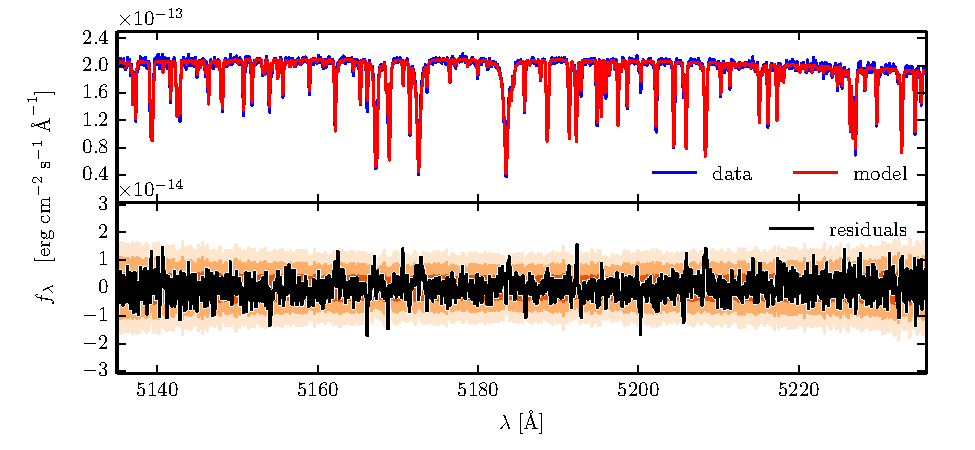
\includegraphics{figs/residuals_Kurucz_logg.pdf}
\caption{Kurucz WASP-14. One, two, and three sigma contours formed from 200 random draws from the covariance matrix.}
\label{fig:residuals_Kurucz}
\end{center}
\end{figure*}

\begin{figure}[!htb]
\begin{center}
  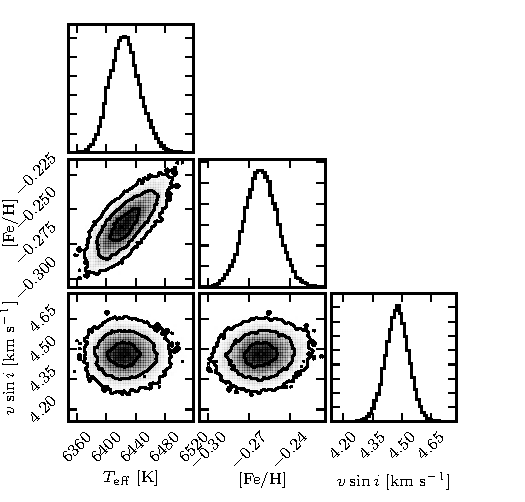
\includegraphics[width=0.5\textwidth]{figs/Kurucz_triangle.pdf}
  \caption{The posterior probability function of the stellar parameters for WASP-14, an F star, as explored by the MCMC Gibbs sampler. These stellar parameters are marginalized over the Chebyshev ($\cheb$) and noise parameters ($\cov$). Figure generated with \texttt{triangle.py} \citep{foreman-mackey14}.
}
\label{fig:stellar_posterior}
\end{center}
\end{figure}

\begin{deluxetable}{lr@{$\pm$}l} 
\tablecaption{\label{table:Kurucz}WASP-14 {\sc CfA/Kurucz} results}
\tablehead{\colhead{Parameter} & \multicolumn{2}{c}{Value}}
\startdata
\cutinhead{Stellar parameters}
$T_{\rm eff}$ & 6517.1 & 12.5 K \\
$\log_{10} g$ & \multicolumn{2}{c}{4.29 dex} \\
$\Z$ & -0.27 & 0.01 dex \\
$v \sin i$ & 4.29 & 0.05 $\kms$\\
$v_z$ & -4.620 & 0.016 $\kms$ \\
$\log_{10} \Omega$ & -12.7181 & 0.0004 \\
\cutinhead{Order 22 nuisance parameters}
$\log_{10} \cc{22}{0}$ &  0.0085 & 0.0005\\
$\cc{22}{1}$ & -0.0142 & 0.0015\\
$\cc{22}{2}$ & -0.0145 & 0.0017\\
$\cc{22}{3}$ & -0.0031 & 0.0011\\
\\
$b_{22}$ & 1.04 & 0.02 \\
$\log_{10} a_{{\rm g}, 22}$ & -14.63 & 0.020 $\textrm{erg}\;\textrm{cm}^{-2}\;\textrm{s}^{-1}\;\textrm{\AA}^{-1}$\\
$l_{22}$ & 7.54 & 0.77 $\kms$ \\

\cutinhead{Order 23 nuisance parameters}
$\log_{10} \cc{23}{0}$ & 0.0030 & 0.0006 \\
$\cc{23}{1}$ & -0.0133 & 0.0016 \\
$\cc{23}{2}$ & -0.0247 & 0.0014 \\
$\cc{23}{3}$ &  0.0012 &  0.0013\\
\\
$b_{23}$ & 1.01 & 0.02 \\
$\log_{10} a_{{\rm g}, 23}$ & -14.55 & 0.015 $\textrm{erg}\;\textrm{cm}^{-2}\;\textrm{s}^{-1}\;\textrm{\AA}^{-1}$\\
$l_{23}$ & 6.52 & 0.50 \\

\cutinhead{Order 24 nuisance parameters}
$\log_{10} \cc{24}{0}$ & \multicolumn{2}{c}{0.00} \\
$\cc{24}{1}$ & -0.0103 & 0.0016 \\
$\cc{24}{2}$ & -0.0112 & 0.0013\\
$\cc{24}{3}$ &  0.0002 & 0.0012\\
\\
$b_{24}$ & 1.02 & 0.02 \\
$\log_{10} a_{{\rm g}, 24}$ & -14.61 & 0.02 $\textrm{erg}\;\textrm{cm}^{-2}\;\textrm{s}^{-1}\;\textrm{\AA}^{-1}$\\
$l_{24}$ & 7.33 & 0.59 $\kms$ \\
\enddata
\end{deluxetable}

\begin{figure}[!htb]
\begin{center}
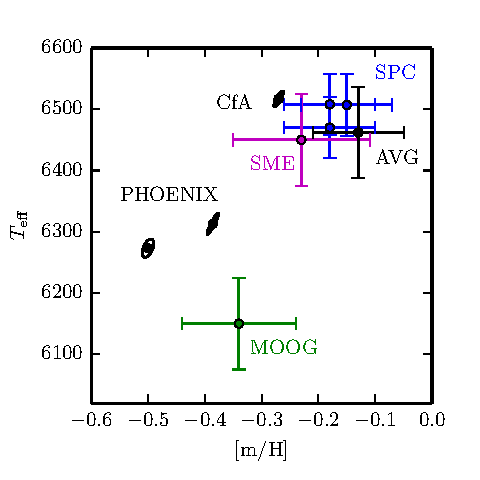
\includegraphics{figs/metacomparison.pdf}
\caption{Comparing all the posteriors.}
\label{fig:metacomparison}
\end{center}
\end{figure}

\comm{Ok, this is where you went off the rails a little bit in the core-dump.  I frankly do not 
want to see Table 2 in this paper, or any reference to specific model or test identifications.  It 
is too confusing, and it obscures the key points we want to make.  I appreciate your desire to 
demonstrate the complexity of the model sequentially, but it does not add anything useful/tangible 
here: it is already done very well in Section 2.  I feel like up to here we have 
established ``reproducibility" well.  The remainder of this section should be solely about 
systematics.  First, I want a paragraph breaking down the origins of the uncertainties (see the 
paragraph I commented out below...I don't like it, but it should give you an idea about what I 
mean.  If I interpret your Google tables correctly, you're getting about half the uncertainty from 
Poisson noise, and the other half from the global covariance kernel.  This is where you need to be 
able to defend the seemingly small uncertainties you're finding, even with a non-trivial covariance 
matrix.  Is it really true that a model with 0.03\,dex lower metallicity cannot describe the data 
as well?  Why?  [This is not to say I don't believe it, but it {\it will} raise questions...]}

Given the apparent differences in the quoted precisions, it is beneficial to review what factors 
into the parameter uncertainties.  In our approach, we consider contributions from both trivial 
(Poisson) noise and a non-trivial Gaussian process covariance matrix.\footnote{It is worth noting 
that the {\sc CfA/Kurucz} library is so good for stars like WASP-14 over this limited spectral 
range that no local covariance kernels need to be instantiated; in this specific case we use only a 
global covariance kernel.}  To break down their respective contributions, we performed the 
same analysis with only a trivial covariance matrix ($b = 1$; $\cov = 0$), which simplifies the 
likelihood function to the familiar $\chi^2$ form.  Doing this, we identify little bias to the 
best-fit parameters, but find unrealistic precision (i.e., $T_{\rm eff}$ to $\pm$5\,K, 
$[{\rm Fe/H}]$ to $\pm0.004$\,dex, and $v \sin i$ to $\pm0.01$\,km s$^{-1}$).  Such small 
uncertainties are to be expected, since the prescribed likelihood function presumes that the data 
are generated from the model; in this paradigm, the only way to introduce deviation is through 
white noise.  Of course, that implicit assumption is invalid, since just a few simple parameters 
($\vT$) are generally insufficient to perfectly account for the thousands of pixels and hundreds of 
spectral features in a typical dataset.  In essence, the data and an imperfect model spectrum also 
have {\it systematic} differences that contribute to the uncertainties (in addition to the Poisson 
noise), which we forward-model using a non-trivial covariance matrix.  In this specific case, these 
systematic uncertainties and the Poisson uncertainties contribute roughly equally to the $\vT$
posteriors.  

\comm{Next, you want to address the observational systematics issue.  Willie (and basically 
everyone else) add empirically-estimated systematic terms in quadrature that make some pretty 
unjustified assumptions: namely that they are Gaussian and independent in each parameter.  If I 
understant Willie's paper correctly, there are 4 TRES observations of WASP-14.  If that is true, I 
think we need to fit each of them independently.  I'd like to know what ``systematic" scatter you 
would derive if you wanted to employ the standard approach.  My gut tells me that it's important to 
simultaneously model all 4 spectra in orders 22-24, but if you think that's not 
computationally tractable, we can discuss more.}
%It is important to note that this ability to parameterize the quality of fit \emph{self-consistently} is unique to a hierarchical Bayesian model, contrary to systematic error estimates that are added in post-facto (I probably don't want to name names, but e.g., \citealt{torres12, buchhave12}). Because the parameter uncertainty is derived through the model itself, it \emph{preserves correlations} between parameters, like the well known degeneracies between $T_{\rm eff}$, $\log g$, and $\Z$. Arbitrarily inflating the posterior estimates to reflect intuition would artificially destroy any natural degeneracy of parameters.  

\comm{Finally, you can transition into the model systematics issue.  Here you want to do the 
modeling for Phoenix in orders 22-24 and demonstrate that you get much different parameters.  You 
will have to show the results, and then can take that opportunity to discuss the local covariance 
kernels.  Just show the results and make these two points, don't belabor the details: I don't 
know what to make of the weird Phoenix parameters.}

\begin{figure*}[!htb]
\begin{center}
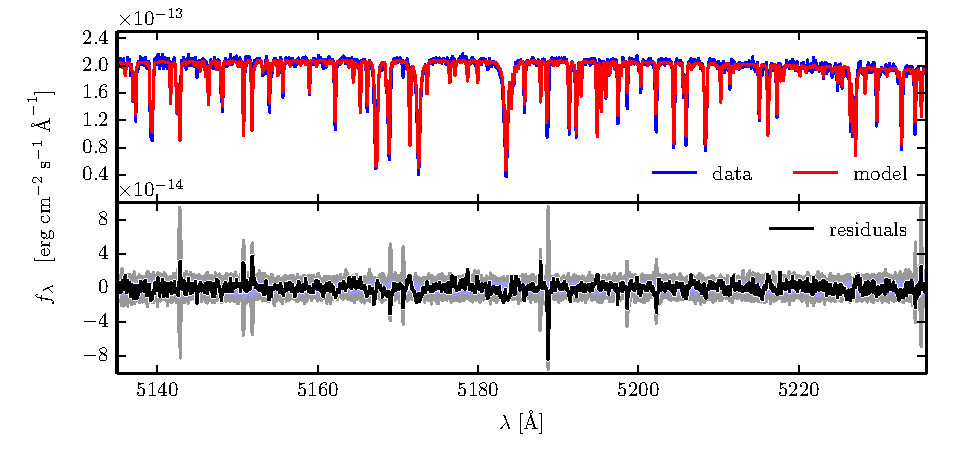
\includegraphics{figs/residuals_PHOENIX_logg.pdf}
\caption{Kurucz WASP-14.}
\label{fig:residuals_PHOENIX}
\end{center}
\end{figure*}


\begin{deluxetable}{lr@{$\pm$}l} 
\tablecaption{\label{table:PHOENIX}WASP-14 {\sc Phoenix} results}
\tablehead{\colhead{Parameter} & \multicolumn{2}{c}{Value}}
\startdata
\cutinhead{Stellar parameters}
$T_{\rm eff}$ & 6516.8 & 12.6 K \\
$\log_{10} g$ & \multicolumn{2}{c}{4.29 dex} \\
$\Z$ & -0.27 & 0.01 dex \\
$v \sin i$ & 4.29 & 0.05 $\kms$\\
$v_z$ & -4.62 & 0.02 $\kms$ \\
$\log_{10} \Omega$ & -12.72 & 0.0004 \\
\cutinhead{Order 22 nuisance parameters}
$\cc{22}{0}$ & & \\
$\cc{22}{1}$ & & \\
$\cc{22}{2}$ & & \\
$\cc{22}{3}$ & & \\
$b_{22}$ & & \\
$a_{{\rm g}, 22}$ & & \\
$l_{22}$ & & \\
\cutinhead{Order 23 nuisance parameters}
$\cc{23}{0}$ & & \\
$\cc{23}{1}$ & & \\
$\cc{23}{2}$ & & \\
$\cc{23}{3}$ & & \\
$b_{23}$ & & \\
$a_{{\rm g}, 23}$ & & \\
$l_{23}$ & & \\
\cutinhead{Order 24 nuisance parameters}
$\cc{24}{0}$ & & \\
$\cc{24}{1}$ & & \\
$\cc{24}{2}$ & & \\
$\cc{24}{3}$ & & \\
$b_{24}$ & & \\
$a_{{\rm g}, 24}$ & & \\
$l_{24}$ & & \\
\enddata
\end{deluxetable}

\comm{I am not sure how/if it will fit in, but I want to see the results of fitting many more 
orders with Phoenix.}

%While the CfA grid spectra fit well with no obvious features in the residual spectrum, because the PHOENIX spectrum is computed over a very broad spectral range and there is no tuning for specific stars like the Sun, there are often a small amount of  ``outlier'' lines that appear in the residual spectrum (e.g., \citealt{husser13}, Figure 8). For demonstrative purposes, for the next test (WP2) we use the common technique of ``sigma-clipping,'' whereby we manually mask any region of the spectrum which has a more than a 3 sigma residual near the best fit parameters, refit, and then proceed until there are no more outliers. Masking out ``outlier'' spectral lines has the effect of actually changing the final stellar estimate significantly, while also reducing the uncertainty in the stellar parameters. However, several questions arise about the quality of the inference on the stellar parameters. Because sigma-clipping is a procedure, it is impossible to quantify the effect that clipping a given line has on the final parameter estimates \citep{hogg10}. For example, what if a series of lines with $\sim$3 sigma disagreement actually has substantial discriminatory power against the stellar parameters? Clipping these lines would discard important information and lead to an incorrect inference of stellar parameters.

%These results motivate the development of a more sophisticated likelihood function which includes a mechanism to account for the systematic mismatch of data spectrum and model spectrum. For the next tests, (WK2 and WP3), we introduce the global covariance kernel (Eqn.~\ref{eqn:global}) to the fit. We can see that the amplitude and scale of the global covariance grows to capture the discrepancy between data spectrum and synthetic spectrum. Including this global covariance broadens the posteriors on the stellar parameters, providing cushion against the tyranny of too many lines, which cause the unreasonably low uncertainty of the previous tests. Therefore, including the global covariance acts as a way to parameterize the goodness or badness of a fit: better spectral models will have a lower covariance, as evidenced by the Kurucz ($10^{-14.6}$) v. PHOENIX ($10^{-14.2}$) global covariance amplitudes. \todo{Figure out a reasonable way to present nuisance parameter values}. It is important to note that this ability to parameterize the quality of fit \emph{self-consistently} is unique to a hierarchical Bayesian model, contrary to systematic error estimates that are added in post-facto (I probably don't want to name names, but e.g., \citealt{torres12, buchhave12}). Because the parameter uncertainty is derived through the model itself, it \emph{preserves correlations} between parameters, like the well known degeneracies between $T_{\rm eff}$, $\log g$, and $\Z$. Arbitrarily inflating the posterior estimates to reflect intuition would artificially destroy any natural degeneracy of parameters.  



%For the next tests, (WPX), we introduce the local covariance kernels to track outlier spectral lines. These kernels can map out the regions of the spectrum which are outliers. The glory of these local kernels are that the parameters allow to play a role in data driven spectra. \emph{A priori} we do not know which regions of the spectrum are improperly modeled. The covariance hyperparameters provide a framework to identify these regions iteratively and in a self-consistent manner.  See Figure~\ref{fig:regions} for a cool visualization of what it looks like. \todo{Runs are almost converged. This can feed into a discussion about tweaking models.}


%In addition to the stark contrast of stellar posteriors derived using only white Poisson noise versus those with the covariance kernels, the results in Table~\ref{table:tests} also reflect the systematic bias that is a function of which spectral library is used as a backend. Depending on your assumptions, there may be systematic differences of 200K or more in $T_{\rm eff}$. 



\subsection{Gl~51}

% Data description of Gl 51
A moderate resolution ($R\approx2,000$) near-infrared spectrum of Gl~51 was obtained on 2000 
Nov 6 using the SPEX instrument \citep{rayner03} on the 2.3\,m NASA Infrared Telescope Facility 
(IRTF).  SPEX is a cross-dispersed echelle that covers the red-optical to thermal-infrared spectrum 
(0.7--5.5\,$\mu$m) in two spectrograph settings.  These data were obtained as part of the IRTF 
spectral standard library project \citep{cushing05,rayner09}, and were processed through the 
well-vetted {\tt Spextool} pipeline \citep{cushing04,vacca03} to deliver a fully-calibrated 
spectrum.  At 2.1\,$\mu$m, the S/N is $\sim$400 per resolution element.

Modeling late-type stellar atmosphere structures and their spectra is considerably more complex 
than for Sun-like stars, due to lingering uncertainties in the atmosphere physics and molecular 
opacities, as well as the presence of complex condensates (clouds) at the coolest temperatures.  
\comm{should probably add some citations to that statement.  Make a comment recognizing that 
various approaches have been taken, in context of Mann.}  \citet{rojas-ayala12} used a $K$-band 
spectrum at similar resolution to the SPEX data to estimate the key Gl~51 stellar parameters based 
on a line index technique.  They measured equivalent widths for the 2.205\,$\mu$m \ion{Na}{1} 
doublet and 2.263\,$\mu$m \ion{Ca}{1} triplet, along with a pseudo-continuum index defined over 
three narrow passbands, 2.070--2.090, 2.235--2.255, and 2.360--2.380\,$\mu$m (see their Figure 2 
for a useful visualization), designed to probe the spectral curvature induced by H$_2$O absorption 
bands.  With reference to a custom grid of {\sc BT-Settl} spectra, \citet{rojas-ayala12} find that 
these indices are consistent with $T_{\rm eff} = 3039\pm56$\,K and $[{\rm Fe/H}] = 0.28\pm0.17$.  

\comm{Now, present your results in a format that parallels the WASP-14 subsection.  You need a new 
Table and a sequence of figures; introduce them all here.}

\comm{Commentary on the necessity and utility of local covariance kernels here, with discussion of why Na and Ca 
lines are a pain.  It is also worth commenting on the potential for flexibly extending the shape of 
the kernel to mimic molecular bandheads, if one wanted to try and fit say the TiO bands.}
%In order to calibrate these indices to stellar parameters, \citet{rojas-ayala12} determine these indices on a custom grid of PHOENIX BT-Settl models obtained from the PHOENIX web simulator\footnote{\url{http://phoenix.ens-lyon.fr/simulator/index.faces}}. They note that the BT-Settl models manage to fit the overall spectral shape well, but consistently under-predict the strength of the \ion{Na}{1} and \ion{Ca}{1} lines, even when using the highest metallicity models. \citet{rajpurohit10} speculate that this discrepancy may result from inaccuracies in the oscillator strengths and opacities for the \ion{Na}{1} and \ion{Ca}{1} lines. When modelling the same region of spectrum as \citet{rojas-ayala12} (2.070--2.380$\mu$m) using an updated set of PHOENIX models \citep{husser13}, we find that 

\begin{figure*}[!htb]
\begin{center}
  \includegraphics[draft,width=0.9\textwidth,height=3in]{figs/Gl51_residuals.pdf}
  \caption{The spectrum residuals and many random draws from the final covariance matrix showing how the uncertainty in the ``outlier'' lines is identified by the local covariance kernels. Plotted with the increased variance envelope over the residuals.}
\label{fig:regions}
\end{center}
\end{figure*}

\begin{figure}[!htb]
\begin{center}
  \includegraphics[draft,width=0.45\textwidth,height=3in]{figs/Gl51_posterior.pdf}
  \caption{The spectrum residuals and many random draws from the final covariance matrix showing how the uncertainty in the ``outlier'' lines is identified by the local covariance kernels. Plotted with the increased variance envelope over the residuals.}
\label{fig:gl_posterior}
\end{center}
\end{figure}

\begin{deluxetable}{lr@{$\pm$}l} 
\tablecaption{\label{table:PHOENIX}Gl51 {\sc Phoenix} results}
\tablehead{\colhead{Parameter} & \multicolumn{2}{c}{Value}}
\startdata
\cutinhead{Stellar parameters}
$T_{\rm eff}$ &  &  K \\
$\log_{10} g$ & \multicolumn{2}{c}{5.0 dex} \\
$\Z$ &  &  dex \\
$v \sin i$ &  &  $\kms$\\
$v_z$ &  &  $\kms$ \\
$\log_{10} \Omega$ &  & \\
\cutinhead{Nuisance parameters}
$\cc{22}{0}$ & & \\
$\cc{22}{1}$ & & \\
$\cc{22}{2}$ & & \\
$\cc{22}{3}$ & & \\
$b$ & & \\
$a_{\rm g} $ & & \\
$l$ & & \\
\cutinhead{Local kernel parameters}
& & \\
& & \\
& & \\
\hline\\
& & \\
& & \\
& & \\
\hline\\
& & \\
& & \\
& & \\
\enddata
\end{deluxetable}

\comm{A simple two-sentence (or so) wrap up on the future promise of this approach for late-type 
stars and their complex spectra.}

\begin{figure}[!htb]
\begin{center}
  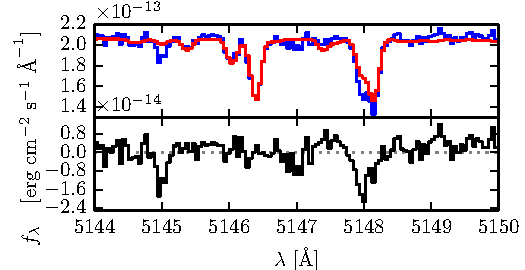
\includegraphics{figs/badlines0.pdf}
  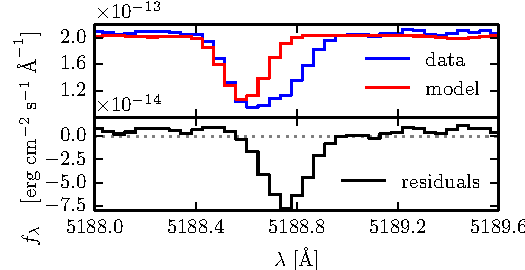
\includegraphics{figs/badlines1.pdf}
  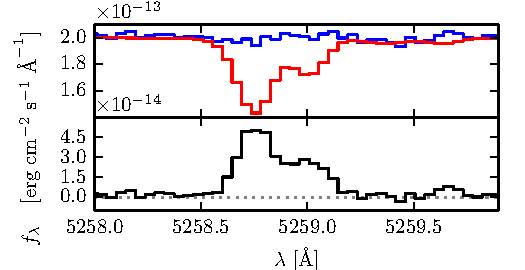
\includegraphics{figs/badlines2.pdf}
  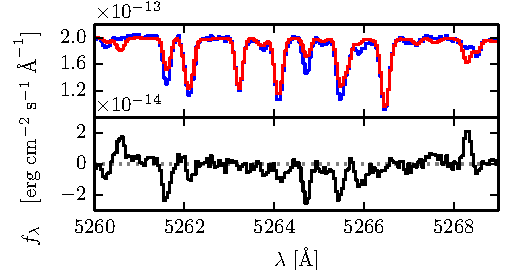
\includegraphics{figs/badlines3.pdf}
  \caption{A collection of spectral lines which have imperfect model fits.
    \textbf{First panel} The majority of spectral lines ($\gtrsim 60$\%) will
    have minor differences in strength between data and model spectrum, which
    produce low-amplitude correlations in the residuals on the length scale of
    the width of a typical spectral line.  \textbf{Second panel}: Sometimes
    ($\lesssim 5$\% of all lines), a missing opacity source in the model (in
    this case a line-blended \ion{Ca}{2}) leaves a large, highly correlated
    patch of negative residuals.  \textbf{Third panel}: Sometimes ($\lesssim
    5$\% of all lines), an extraneous line in the model leaves a large, highly
    correlated patch of positive residuals. \textbf{Fourth panel}: If the line
    strengths are substantially discrepant ($\lesssim 10$\% of all lines),
    there will be many correlated residuals of moderate amplitude.  The
    difficulty with class III lines is that for any specific line, there might
    exist a $\vT$ that will fit the line, but there does not exist a $\vT$ that
    will properly fit \emph{all} the lines.}
\label{fig:badlines}
\end{center}
\end{figure}

\section{Discussion}
\label{sec:discussion}
%\begin{rant about why this method rocks}
There are many advantages to placing spectroscopic inference within a Bayesian framework. Given the large costs of acquiring a high signal to noise spectrum, it would be advantageous to utilize as much as possible of the spectrum for performing inference. You go to a telescope to take a spectrum, you should use the whole spectrum, not just subsets of the spectrum that are certain well chosen lines. True, these lines have been identified by the accumulated knowledge of experts to show high discriminatory power against the stellar parameters of interest, but there is a gap in the chain of logic between these indices and the core fundamental physics knowledge, since calibrations must still be derived against synthetic models. These ``fit metrics'' (line indices) are similar to distance functions or a figure of merit.

These figures of merit do make a lot of sense, and one can see why they are used, but given that the raw data product from synthetic models from stars is \emph{actually a spectrum} that has been synthesized from a complicated but \emph{physical} model of a star, instead of going through the intermediary step of a figure of merit, wouldn't it be better to relate the two through an actual \emph{likelihood function}, a physical description of the process that generates the data? In this case we use a Gaussian process to absorb the computational artifacts/inaccuracy that is a result from a \emph{imperfect} (but still extraordinarily good) stellar model. This allows us to couch the question of what parameters does the star have in a truly \emph{probabilistic} framework, meaning, we can calculate a posterior probability function of the parameters that is grounded in our physical understanding of what a star looks like. This is one of the great things about a \emph{forward-model}.

The main advantage of using a more sophisticated hierarchical likelihood function (Eqn~\ref{eqn:likelihood}) than $\chi^2$, is that the model-data mismatch becomes a parameter in the model. When the model is of higher quality, the confidence in the stellar posteriors grows and is reflected by a smaller uncertainty. When the model is of lesser quality, the stellar posteriors inflate to reflect the increased uncertainty in the stellar parameters. This hierarchical model also works within a single spectrum when fitting more than one spectral order. If each order has a disparate prediction about the stellar parameters, then the global kernels will have a low amplitude and the final posterior will be an improved estimate. However, if certain orders predict different stellar parameters, the global kernels will inflate to absorb the model-data mismatch and consequently inflate the posteriors on the stellar parameters.
%\end{rant}

The traditional manner of dealing with spectral mismatch is to simply mask out the regions of the spectrum which do not agree to within a certain tolerance. Rather than arbitrarily excluding regions of the spectrum from the fit, these regions should instead be incorporated into in the fit with the appropriate weight. A model that includes covariance is far more likely than forcing the synthetic spectrum to fit perfectly, and far more flexible than arbitrarily masking regions which do not fit. The fitting procedure allows these weights to be determined self-consistently, such that lines which are slightly wrong can still bring information to bear on the stellar parameters. In fact, for some types of stars with difficult-to-model spectra, it may be possible that the lines that are incorrect by a small amount actually provide the \emph{most information} about the stellar parameters, precisely because these lines are the most sensitive to stellar structure and consequentially are the most difficult to model correctly.

The benefits of using covariance hyperparameters also extend beyond the use case of fitting a single stellar spectrum. If we fit many stars with the same set of synthetic models, we can use the structure of the covariance matrix to improve the models themselves. By cataloguing the covariance structure of the residuals, especially those generated from strong spectral line mismatch, we collect valuable information about the quality of the synthetic spectra. After fitting many stars, the accumulated knowledge of the data-model mismatch can be used when fitting a new star. The previous structure of the covariance matrix allows us to set priors on what the covariance in certain regions of the spectrum should be, which will speed convergence for this new star. Additionally, after fitting several stars, the average value of the covariance matrix will inform us about the quality of specific spectral lines in the synthetic models. 

Linking the covariance matrices of stars could be done serially, where the aggregate covariance matrix of all previous fits is used as a prior for the current iteration. Or, the covariance matrices could instead be linked hierarchically, in that the parameters describing the depth and width of a line residual for a specific star $a_1$ and $\sigma_1$, are modeled as coming from of a population of possible depths and widths for a given spectral type. Each stellar spectrum will have a slightly different realization of a spectral line, which will have some scatter about the average residual height. Linking the covariance matrix between spectra of similar stars allows us to grow more confident in our assessment that certain synthetic spectral lines are indeed outliers and should be appropriately down-weighted. In turn, as we become more certain of the weights, the stellar posteriors will become narrower and make our estimates of the stellar parameters more precise. This ability of the model to mutually inform sets of parameters is one of the major advantages of hierarchical Bayesian analysis \citep{kruschke10}.

Once determined, this average covariance matrix could be delivered to the communities that created the synthetic libraries, which would enable them to rapidly pinpoint and correct non-physical lines in the synthetic models. Alternatively, we could correct the models ourselves by using the chain of logic and mathematical post-processing that we used to created the synthetic model spectrum to reverse-engineer what the behavior of the raw synthetic spectrum \emph{should} be, at the raw $R \gtrsim$~100,000 resolution. This fundamental application of machine learning would enable us to create our own library of data driven, semi-empirical stellar models. Rather than simply assembling an empirical spectral library using only real stellar spectra, this combined approach is more powerful because the synthetic stellar atmospheres provide an actual anchor point of fundamental stellar parameters tied down by the laws of stellar physics.

\todo{We can (should?) add an additional level to the hierarchy of hyperparameters and add parameters to describe the \emph{population characteristics} of poorly modeled spectral lines (mostly the typical width, amplitude of these lines).  This will tell us about the frequency and distribution of spectral modelling errors. Or we could just speculate about it.}

\section{Conclusion}
\label{sec:conclusion}

\bibliographystyle{yahapj}
\bibliography{stellarspectra}

\section{Tables}

\begin{deluxetable}{ll}
\tablecaption{Nomenclature used in this document}
\tablehead{
  \colhead{Symbol} & \colhead{Description}
}
\startdata
$\lambda_i$ & wavelength corresponding to a given pixel $i$\\
$\vt_{\ast}$ & fundamental stellar parameters, $T_{\rm eff}, \log(g), \Z, \A$\\
$\{\vt_{\ast}\}^{\rm grid}$ & stellar parameters that specify a spectrum from a synthetic library\\
$\vt_{\rm obs}$ & stellar parameters $v \sin i$, $v_z$, $A_V$, and $R^2/d^2$ that\\
  & are applied during ``post processing'' of the synthetic spectrum\\
$\vt$ & $\{\vt_{\ast},\vt_{\rm obs}\}$, all stellar parameters\\


$\chebi{i}$ & $\{c_0, c_1, \ldots, c_{n-1}\}$ the set of Chebyshev polynomial coefficients  for \\
 & a single spectral order $i$ \\
$\Cheb$ & $\{\chebi{1}, \chebi{2}, \ldots, \chebi{N} \}$, the collection of all Chebyshev parameters for \\
  & a multi-order echelle spectrum with $N$ spectral orders  \\
 $\Chebi{2}$ & $\{\chebi{1}, \chebi{3}, \ldots, \chebi{N}\}$, the collection of all Chebyshev parameters \\
 & except those for order $2$ \\
$\covi{i}$ & $[a_g, \ell, \{a_k, \mu_k, \sigma_k, h_k\}^{N_{\rm reg}}]$, the set of covariance hyperparameters for a single spectral order $i$ \\
$\Cov$ & $\{ \covi{1}, \covi{2}, \ldots, \covi{N} \}$, the collection of all covariance hyper-parameters for \\
 & a multi-order echelle spectrum with $N$ spectral orders  \\
 $\Covi{2}$ & $\{\covi{1}, \covi{3}, \ldots, \covi{N}\}$, the collection of all covariance hyperparameters \\
 & except those for order $2$ \\

$\vP$ & $\{\Cheb, \Cov \}$, the collection of all nuisance parameters \\
$\vT$ & the collection of all stellar parameters \\
$\vD$ & data spectrum \\
$\vM$ & model, a function of the above stellar, Chebyshev, and covariance (hyper)parameters \\
$\vR$ & $\vD - \vM $, residuals  \\
$\vC$ & covariance matrix, a function of the covariance hyper-parameters\\
$\vC_{ij}$ & an individual element in the covariance matrix\\
$r(\lambda_i, \lambda_j)$ & radial distance in wavelength space corresponding to $\Delta v$\\

$\Kglobal$ & global covariance kernel\\
$\Klocal$ & local covariance kernel\\
$w$ & Hanning taper for kernels \\
\enddata
\end{deluxetable}

\appendix

This version of the paper was generated
 from a git repository available at \url{http://github.com/iancze/StellarSpectra/}
 with git hash \texttt{\githash\,(\gitdate)}.
\end{document}
